\errorcontextlines9999
\documentclass[parskip=half,english,noenddot,numbers=noenddot,footnotes=nomultiple,oneside]{scrartcl}

\usepackage[T1]{fontenc}
\usepackage[utf8]{inputenc}
\usepackage[english]{babel}

\usepackage[glows]{tikzpingus}
\usepackage[linkcolor=pingu@purple,urlcolor=pingu@purple,colorlinks,breaklinks,pdfusetitle]{hyperref}
\urlstyle{same}
\expandafter\def\expandafter\UrlBreaks\expandafter{\UrlBreaks\do-}

\usepackage[tex,hyper]{listings}
\usepackage[most]{tcolorbox}
\usepackage{imakeidx,tikz,fontawesome,csquotes,enumitem,microtype,tikzducks,datatool,relsize,multicol,footnotebackref,adjustbox}
\makeindex[title={Key Overview},columns=2,columnsep=.75cm,noautomatic=true]
\deffootnote{1.5em}{1em}{\textsuperscript{\hyperref[\BackrefFootnoteTag]{\thefootnotemark}}\thinspace}
\def\thefootnote{$\langle$\arabic{footnote}$\rangle$}

\newlist{inlist}{enumerate*}{1}
\setlist[inlist]{itemjoin={{,\space}},itemjoin*={{, and }},label=$\roman*$),mode=boxed}
\let\say\enquote
\def\DTLlistformatoxford{,}
\def\DTLandname{and}
\def\DTLlistformatitem#1{\textit{#1}}
\newcommand*\typesetselection[1][]{\begingroup\ifx!#1!\else\def\DTLlistformatitem##1{#1}\fi\dotypesetselection}
\def\dotypesetselection#1{\expandafter\DTLformatlist\expandafter{\csname @pingu@#1@\endcsname}\endgroup}
\usepackage{lmodern,CrimsonPro}
\makeatletter

\addtokomafont{sectioning}{\color{gray}}
\addtokomafont{title}{\color{pingu@purple}}
\addtokomafont{author}{\normalsize}
\addtokomafont{date}{\normalsize}

\def\optstyle{\color{pingu@blue!75!black}\slshape}
\lstdefinestyle{lstpingu}{%
	tabsize=2, breaklines,
	basicstyle=\relsize{-.8}\ttfamily,
	commentstyle={\color{gray}\slshape},
	columns=fullflexible,
	emphstyle=\slshape,
	emphstyle=[2]\optstyle,
	emphstyle=[3]\color{gray!75!white},
	emphstyle=[4]\color{pingu@blue!40!black},
	texcsstyle=*\color{gray}\bfseries,
	texcsstyle=*[2]\color{pingu@purple}\bfseries,
	lineskip=2.75pt,
	keepspaces=true,
	moredelim=[s][\itshape]{<}{>},
}
\lstset{style=lstpingu}
\def\ipingu#1{\lstinline'#1'}
\def\lpingu#1{\lstinline[style=lstpingu,language=pingulang]'#1'}

\def\t@lst@addToLiterate#1{\protected@edef\lst@literate{\unexpanded\expandafter{\lst@literate}\unexpanded{#1}}}
\lst@Key{add to literate}{}{\t@lst@addToLiterate{#1}}

\lstdefinelanguage{pingulang}{
	language={[LaTeX]TeX},
	moreemph={tikzpicture},
	alsoletter={.-!:0123456789},%disable number
	moreemph=[2]{left,right,wing,eye,wings,tie,bow,none,eyes,shiny,wink,wave,grab,hug,wave,cup,straw,xshift,yshift,meta,dots,name,heart,shock,bill,hair,hairstyle,feet,foot,simple,flat,angry,back,devil,normal,princess,crown,silver,medal,patch,halo,glow,thick,2d,sunglasses,gem,shade,round,lollipop,lightsaber,item,angle,raise,cane,flip,flag,sign,post,cloak,scale,meta-dots,color,body,head,main,front,second,height,small,size,large,style,hairs,1,2,3,4,5,knot},
	moreemph=[4]{:line,:ghost,parts,:devil,:back},
	moretexcs=[2]{pingu,duck,node,pingudefaults,pingudefaultsappend},
	moreemph=[3]{!hide},
	add to literate={/pingu/}{{\textcolor{gray}{/pingu/}}}7
}
\NewEnviron{scaleme}[1]{\scalebox{#1}{\BODY}}

\tcbset{%
	colframe=gray,enhanced,breakable,
	arc=2mm, arc is angular,
	fonttitle=\bfseries,
	sidebyside,
	listing options={style=lstpingu,language=pingulang},
	center lower,
	righthand width=5cm,
	bottom=0pt,top=0pt,
	before lower app={\parskip.5cm},
}
\lstMakeShortInline[style=lstpingu]{|}

\def\explaincolor{pingu@purple!8!white}
\def\cursub{}
\newenvironment{keyexplain}[4][/pingu/]{\begin{minipage}{\linewidth}%
	\parskip\medskipamount
	\phantomsection\label{pk:#1#2}\index{\cursub#2?\hyperref[pk:#1#2]{\lpingu{#2}}}%
	\expandafter\gdef\csname pinguopt#2\endcsname{#3}%
	\expandafter\gdef\csname pingudefa#2\endcsname{#4}%
	\begingroup\pgfkeys{/pingu/.cd,defaults}\protected@edef\@tmp{#4}%
	\protected@edef\@tmpb{#3}%
	\hspace*{-2em}\colorbox{\explaincolor}{%
		\parbox{\dimexpr\linewidth-2\fboxsep+2em}{\small%
		\ifx\@tmpb\@empty\lpingu{#1#2}\else\lpingu{#1#2 =\ }\texttt{<\textit{\@tmpb}>}\fi\hfill
				\ifx\@tmp\@empty\else\textcolor{gray}{(}#4\textcolor{gray}{)}\fi%
		}
	}\\*[\smallskipamount]\endgroup}
{\end{minipage}\medskip\par}

\def\singleshortcut#1#2#3#4{\def\cursub{#2?\hyperref[pk:#1#2]{\lpingu{#2}}!}\begin{keyexplain}[#1]{#2 #3}{\csname pinguopt#4\endcsname}{\csname pingudefa#4\endcsname}%
	\textcolor{gray}{\footnotesize This is a shortcut for: \texttt{\keyref[#1]{#2} = {\optstyle#3}}. The \enquote{\texttt{\textit{\csname pinguopt#4\endcsname}}} argument is passed to the key \keyref[#1]{#4}.}
\end{keyexplain}}
\newcommand*\shortcuts[4][/pingu/]{\begingroup
\protected@edef\@tmp{#3}%
\def\explaincolor{gray!10!white}%
\foreach \type in \@tmp {%
\edef\tmp{\noexpand\singleshortcut{#1}{#2}{\type}{#4}}\tmp
}\endgroup}

\newcommand*\keyref[2][/pingu/]{\hyperref[pk:#1#2]{\lpingu{#1#2}}}

\newenvironment{subkeyexplain}[5][/pingu/]{%
\begingroup
\def\explaincolor{gray!10!white}%
\def\cursub{#2?\hyperref[pk:#1#2]{\lpingu{#2}}!}%
\begin{keyexplain}[#1]{#3}{#4}{#5}%
	\textcolor{gray}{\footnotesize This command is only active in combination with \keyref[#1]{#2}.}\par
}{\end{keyexplain}\endgroup}

\newcommand{\keyalias}[3][/pingu/]{\begingroup
\def\explaincolor{gray!10!white}%
\def\cursub{#3?\hyperref[pk:#1#3]{\lpingu{#3}}!}%
\begin{keyexplain}[#1]{#2}{\csname pinguopt#3\endcsname}{\csname pingudefa#3\endcsname}%
	\textcolor{gray}{\footnotesize This is an alias for \keyref[#1]{#3}.}%
\end{keyexplain}\endgroup}

\def\TikZ{Ti\textit{k}Z}
\def\tikzpingus{\TikZ pingus}

\title{The \texorpdfstring{\tikzpingus}{tikzpingus} package}
\subtitle{penguins in \TikZ}
\author{%
	\texorpdfstring{Florian Sihler\\[.4em]
		\url{https://github.com/EagleoutIce/tikzpingus}
	}{Florian Sihler}}
\date{Version v1.0 \textendash\ 2021/07/02}

\begin{document}
\maketitle

\section{Motivation}
For my slides at university, I started to use the fairly famous \LaTeX-package \textsl{\href{https://github.com/samcarter/tikzducks}{tikzducks}} a few years ago.
Yet, it seemed somewhat of a necessity to extend the range of available \say{cute} animals in \LaTeX.
Therefore I started writing this package: \textsl{tikzpingus}.\footnote{Why \say{pingu} and not \say{pengu}? Well, this is the third try on achieving cute penguins without using any templates or vector formats as a basis. As a german, the short form \say{pingu} was merely a typo that originated from the german word \say{pinguin} for \say{penguin}. It somewhat sticked\ldots}

\textit{Please note:} While tikzpingus is certainly inspired by tikzducks, it does offer a different set of features (e.g. multiple arm positions,~\ldots).

I would be happy for any feedback or issues on the \href{https://github.com/EagleoutIce/tikzpingus}{tikzpingus}-GitHub.

\subsection{Dependencies}

As this package is constantly work in progress, the concrete dependencies may change any time.
At the moment, it only loads \TikZ, which loads a lot of other packages (e.g. |xcolor|).
Furthermore, the following \TikZ-Libraries are in use:\footnote{A lot of the libraries loaded are important only for specific extras. I plan on cleaning them up.}
\begin{inlist}
	\item |intersections|
	\item |shadings|
	\item |patterns.meta|
	\item |decorations.pathmorphing|
	\item |shapes.symbols|
\end{inlist}.

\subsection{Copyright}

Copyright \textcopyright\ \texttt{Florian Sihler}. Permission is granted to copy, distribute and\slash or modify this software under the terms of the LaTeX project public licence, version 1.3c or later \url{http://www.latex-project.org/lppl.txt}.

The shown example penguins are purely fictional characters, any resemblance to real penguins or persons is purely coincidental and no copyright infringement is intended.

\section{Usage}

If you just want a penguin, use the following syntax:
\begin{tcblisting}{title={One small penguin}}

\begin{tikzpicture}
	\pingu
\end{tikzpicture}
\end{tcblisting}

There are \textit{a lot} of configuration-options which can be passed as an optional argument via the known |<key>=<value>|-style.
% TODO: click reference to full list; TODO: glow option
\begin{tcblisting}{title={Happy penguin with cup!}}
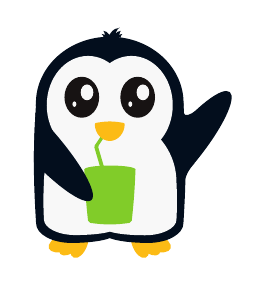
\begin{tikzpicture}
	\pingu[left wing wave, right wing grab,
	       eyes shiny, cup]
\end{tikzpicture}
\end{tcblisting}
Please note, that \say{left} and \say{right} have been chosen from the penguin-perspective.

Besides the keys defined by this package, you can use the keys of \TikZ\ and |pgf| as well (the duck was generated by the lovely \href{https://github.com/samcarter/tikzducks}{tikzducks} package):
\begin{tcblisting}{title={The Reunion}}
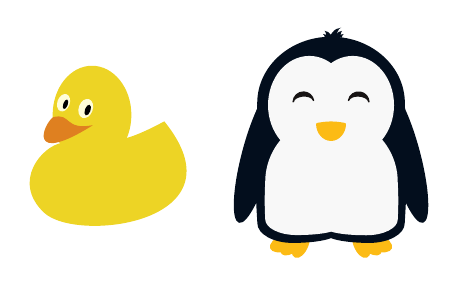
\begin{tikzpicture}
	\duck
	\pingu[xshift=3cm, yshift=14mm,
	       eyes wink]
\end{tikzpicture}
\end{tcblisting}
\subsection{Using the Coordinates}
\label{mrk:coordinates}While there are a lot of gadgets available already,
every penguin is accompanied by \textit{a lot} of adaptive coordinates
to place custom items, texts,~\ldots\ % TODO: links
They can be placed by the meta-dots option and change their positions, angles,~\ldots\ depending on other options.
Furthermore, some extras create further coordinates themselves!
All coordinates are available with |<pigu-name>-<coordinate>|.
While the default name of a penguin is \say{pingu}, it can be
changed with the name option:
\begin{tcblisting}{title={Lotta dots}}
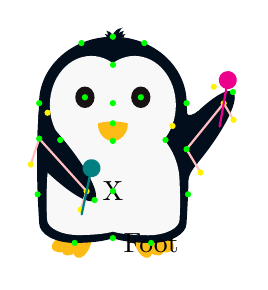
\begin{tikzpicture}
	\pingu[meta dots,left wing wave,
	       right wing grab, name=paula]
	\node at (paula-belly-center) {X};
	\node at (paula-foot-left) {Foot};
\end{tikzpicture}
\end{tcblisting}
Lets look at those coordinates in more detail (all labels are to be prefixed by |<pingu-name>-|):
\newsavebox\pinguwingright
\savebox\pinguwingright{%
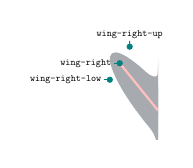
\begin{tikzpicture}%
	\scope
	\path[clip] (0,-.7) rectangle (-1,.7);
	\pgfonlayer{foreground}\path[clip] (0,-.7) rectangle (-1,.7);\endpgfonlayer
	\pingu[@block/.append style={fill=#1!35!white}, wings wave,eyes shiny,heart=gray!30!white,feet=none]
	\path[draw,pink,thick] (pingu-wing-right-start) -- (pingu-wing-right);
	\endscope
	\foreach \c/\a in {wing-right/left,wing-right-low/left,wing-right-up/above} {
		\path[fill=teal] (pingu-\c) circle [radius=1.125pt];
		\node[\a=.75mm,font=\ttfamily,scale=.35,inner sep=2.5pt] (expl-\c) at (pingu-\c) {\c};
		\draw[teal,thin] (expl-\c) -- (pingu-\c);
	}
\end{tikzpicture}%
}
\makeatletter
\newsavebox\pinguwingleft
\savebox\pinguwingleft{%
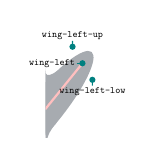
\begin{tikzpicture}%
	\scope
	\path[clip] (\pingu@w@half*2,-.7) rectangle ++(1,1.4);
	\pgfonlayer{foreground}\path[clip] (\pingu@w@half*2,-.7) rectangle ++(1,1.4);\endpgfonlayer
	\pingu[@block/.append style={fill=#1!35!white}, wings wave,eyes shiny,heart=gray!30!white,feet=none]
	\path[draw,pink,thick] (pingu-wing-left-start) -- (pingu-wing-left);
	\endscope
	\foreach \c/\a in {wing-left/left,wing-left-low/below,wing-left-up/above} {
		\path[fill=teal] (pingu-\c) circle [radius=1.125pt];
		\node[\a=.75mm,font=\ttfamily,scale=.35,inner sep=1.5pt] (expl-\c) at (pingu-\c) {\c};
		\draw[teal,thin] (expl-\c) -- (pingu-\c);
	}
\end{tikzpicture}%
}

\begin{center}
	\resizebox{.9\linewidth}!{
		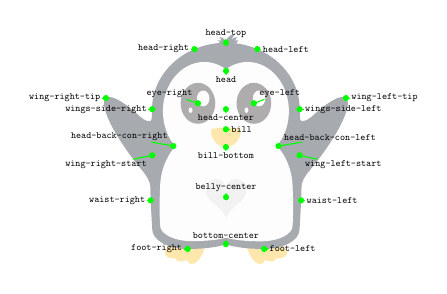
\begin{tikzpicture}
			\pingu[@block/.append style={fill=#1!35!white}, wings wave,eyes shiny,heart=gray!30!white]
			\pgfonlayer{foreground}
			\foreach \c/\a in {belly-center/above,head/below,head-top/above,foot-left/right,foot-right/left,eye-right/above left,eye-left/above right,bill/right,bill-bottom/below,wings-side-left/right,wings-side-right/left,wing-left-start/below right,wing-left-tip/right,wing-right-start/below left,wing-right-tip/left,head-right/left,head-left/right,head-center/below,head-back-con-left/above right,head-back-con-right/above left,bottom-center/above,waist-left/right,waist-right/left} {
				\path[fill=green] (pingu-\c) circle [radius=1.125pt];
				\node[\a=.5mm,font=\ttfamily,scale=.35,inner sep=1.5pt] (expl-\c) at (pingu-\c) {\c};
				\draw[green,thin] (expl-\c) -- (pingu-\c);
			}
			\endpgfonlayer
		\end{tikzpicture}
	}
\end{center}

\paragraph{The Wings}
This view excluded a lot of special data collected on the wings!
While there is more information stored for each wing, the following three coordinates are the most important to place items into penguins hand:
\begin{center}
	\null\hfill\parbox[c]{2.5\wd\pinguwingright}{\scalebox{2.5}{\usebox\pinguwingright}}\hfill\parbox[c]{4cm}{\centering\scriptsize\color{gray}\sffamily And yes, the wings are deliberately placed asymmetrical.\endgraf}\hfill
	\parbox[c]{2.5\wd\pinguwingleft}{\scalebox{2.5}{\usebox\pinguwingleft}}\hfill\null
\end{center}

\subsection{Colors}
A lot of options allow for a color to passed. In general, you can provide any color that \TikZ\ is happy with! Yet, there are some predefined pingu-colors shipped with this package, and there is one special \say{color}:
\begin{multicols}{4}
\begin{itemize}
	\foreach \col in {main,black,silver,bronze,white,yellow,lightblue,blue,green,red,purple} {
		\item[{\tikz[baseline=-.6ex]{\fill[pingu@\col,semithick,draw=black] circle (4pt);}}] \small\texttt{pingu@\col}
	}
	\item[] % buffer
\end{itemize}
\end{multicols}
Furthermore, there is the color {\makeatletter\say{\expandafter\ipingu\expandafter{\@pingu@none}}} which is available for most\footnote{Why just \say{most}? Well, this package is work in progress and I have added the option late, so I may have forgotten to patch some keys.} extras and wing-items. This color prohibits the compartments from being drawn. To be more precise, the package defines the macro |\pingu@none|, which is matched against the selected color.

As an example, lets take a look at the \say{cup}-extra, which provides an additional key \say{cup straw} to color the straw:
\begin{tcblisting}{title={Cup without a straw}}
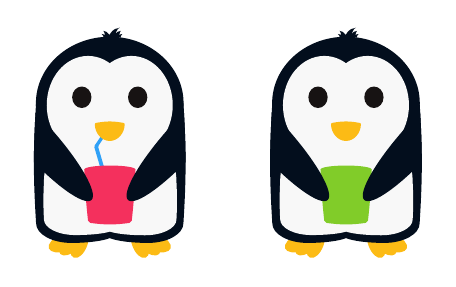
\begin{tikzpicture}
	\pingu[wings grab, cup=pingu@purple,
	       cup straw=pingu@blue]
	\pingu[wings grab, cup, xshift=3cm,
	       cup straw=!hide]
\end{tikzpicture}
\end{tcblisting}

\subsection{Setting the defaults}
You do not have to state every key for every penguin.
With the two macros \lstinline[language=pingulang]'\pingudefaults' and \lstinline[language=pingulang]'\pingudefaultsappend' (works the same, but will extend the current options) you can set default-options for all penguins to come:
\begin{tcblisting}{title={Change the mainstream}}
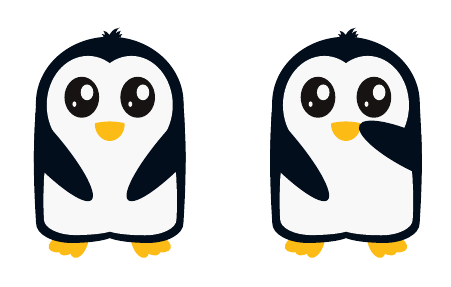
\begin{tikzpicture}
	  tie=pingu@purple
	\pingudefaults{wings grab, eyes shiny,}
	\pingu
	\pingu[left wing shock, xshift=3cm]
\end{tikzpicture}
\end{tcblisting}

\subsection{Changing the wings}
\label{subsec:wings}As already demonstrated, it is possible to change the wing positions!
All selected wing-items will adapt to the wing-position (although not all wing-items will make sense with every wing-position).
Currently, there are the following wing-positions:
\typesetselection{leftwing}. \say{none} is a special wing-position: it omits the drawing of wings (teaser: every selection has a none-option, which prohibits the part from being drawn)!

For each valid wing-position you can use |wings <position>| to change both wings or |left wing <position>| and |right wing <position>| to change only one wing respectively. The default wing-position is \say{normal}. If you supply more than one option for a wing, only the last one will survive.\footnote{For the sake of completeness: \ipingu{wings <position>}, \ipingu{left wing <position>}, and \ipingu{right wing <position>} are just alternatives that i prefer over the underlying mechanism: \ipingu{wings=<position>}, \ipingu{left wing=<position>} and \ipingu{right wing=<position>}.}
\begin{tcblisting}{sidebyside=false, title=Wing-Showcase}
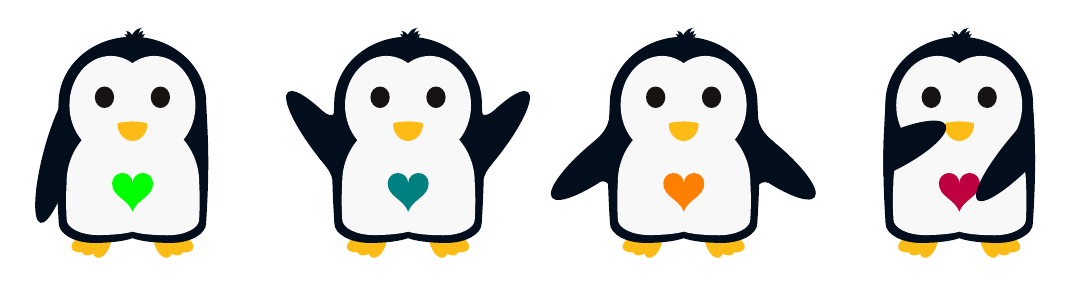
\begin{tikzpicture}
	\pingu[left wing none, heart=green]
	\pingu[wings wave, heart=teal,    xshift=3.5cm]
	\pingu[wings hug,  heart=orange,  xshift=7cm]
	\pingu[left wing grab, right wing shock, heart=purple,  xshift=10.5cm]
\end{tikzpicture}
\end{tcblisting}

\subsection{Changing the eyes}
\label{mrk:pengu-eye}Just like the wings, there are a couple of different eye-styles to choose from: \typesetselection{lefteye}. Just like the wings, there is a \say{none} and a \say{normal}-option (which is the default).
Furthermore, the convenient selectors |eyes <style>|, |left eye <style>|, and |right eye <style>| exist as well:
\begin{tcblisting}{sidebyside=false, title=Eye-Showcase}
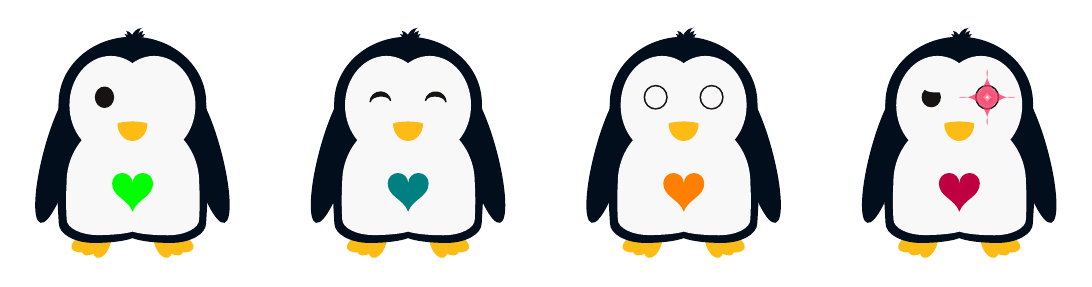
\begin{tikzpicture}
	\pingu[left eye none, heart=green]
	\pingu[eyes wink, heart=teal, xshift=3.5cm]
	\pingu[eyes shock,  heart=orange, xshift=7cm]
	\pingu[left eye devil, right eye angry, heart=purple,  xshift=10.5cm]
\end{tikzpicture}
\end{tcblisting}

\subsection{Changing other components}
\label{mrk:pengu-change-comps}Just like for the wings and the eyes, you can change th following body parts:
\begin{itemize}
	\item The \textit{feet} (again with separate left and right)\\*
		Select from: \typesetselection{leftfoot}.
	\item The \textit{bill} (does not have left and right, as there is just one)\\*
		Select from: \typesetselection{bill}.
	\item The \textit{hairstyle} (does not have left and right)\\*
		Select from: \typesetselection{hairstyle}.
\end{itemize}
For each selection, \say{none} will prohibit the drawing, and \say{normal} is the default chosen.
\begin{tcblisting}{sidebyside=false, title=Bodyparts-Showcase}
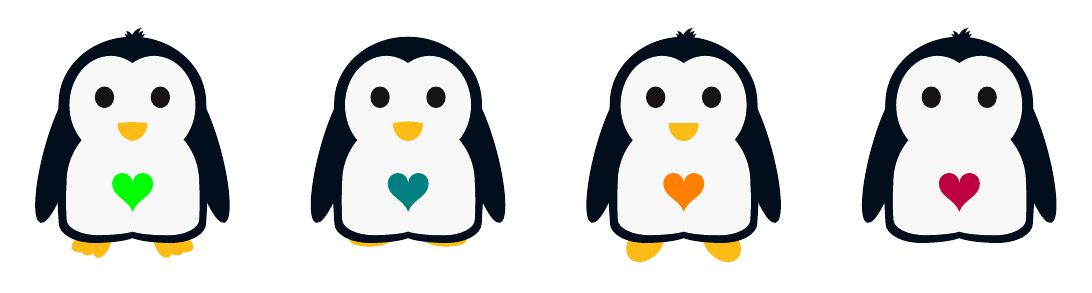
\begin{tikzpicture}
	\pingu[bill angry, heart=green]
	\pingu[feet back, hairstyle none, heart=teal, xshift=3.5cm]
	\pingu[bill flat, feet simple, heart=orange, xshift=7cm]
	\pingu[feet none, bill none, heart=purple, xshift=10.5cm]
\end{tikzpicture}
\end{tcblisting}

\subsection{Predefined Styles}
While the penguin options offer the modification of basically every drawing routine (through other styles like |@block|), it is tedious to change them every time.
So I have started to create some predefined styles, that do change some of the penguins appearance (and are completely new, so beware of bugs):
\begin{multicols}{2}
\begin{itemize}
	\foreach \tx/\s in {{draw everything with a line}/{:line}, {draw components with transparency}/{:ghost parts}, {draw all layers with transparency}/{:ghost}, {set all of the \say{devil}-components}/{:devil},{flip the penguin (swaps left \& right)}/{:back}} {
		\item \parbox[t]{.8\linewidth}{\raggedright\texttt{\s}, \tx.} \hfill
		\parbox[t]{.175\linewidth}{\scalebox{.4}{%
			
\begin{tikzpicture}[baseline=.35\baselineskip]%
				\pingu[\s]
			\end{tikzpicture}%
		}}
	}
	\item[] \parbox[t][2.4\baselineskip]{0pt}{}% buffer
\end{itemize}
\end{multicols}
Currently, only some of the styles do affect other items. As an example, consider |:line|, that changes the draw-style of wing-items and extras:
\begin{tcblisting}{title={Line Penguin}}
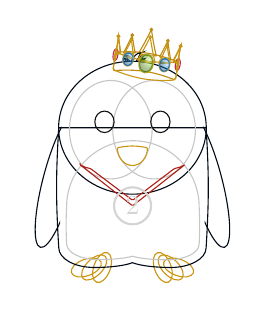
\begin{tikzpicture}
	\pingu[:line, princess crown, silver medal]
\end{tikzpicture}
\end{tcblisting}

\subsection{Extras}
An extra is considered everything, that is attached to the main penguin and not to the wings (as those items may be placed separately for both wings).
Most extras are activated with the format |<extra>=<color>| (the |<color>| option is not mandatory)
and try to adapt with other extras that have been placed (yet you can place multiple hats if you really like to).  A lot of the extras do offer more keys to customize their appearance.
They are explained in the full reference (\autoref{sec:full-ref}).

Consider the following, somewhat overkill-example:
\begin{tcblisting}{title={Lord-Gadget, the penguin}}

\begin{tikzpicture}
	\pingu[crown 2d=pingu@bronze,
	       medal=pingu@purple, tie,
	       eye patch left=teal,
	       eye patch right=orange,
	       right wing wave, sunglasses,
	       glow thick=yellow]
\end{tikzpicture}
\end{tcblisting}

\subsection{Wing-Items}
Wing items are basically just like extras, but they can be selected separately for the left and right wing. Furthermore, they adapt their \textit{default} appearance to the active wing positions (\autoref{subsec:wings}).
Currently there are the following wing items:
\typesetselection{wingitems}.
They are selected using |<wing item> <left/right>|.

Additionally, they can be customized by |<left/right> item angle=<angle>| and |<left/right> item flip=<true/false>|.
Lets consider an example\ldots
\begin{tcblisting}{title={Penguin with full wings!}}

\begin{tikzpicture}[scale=.75]
	\pingu[lightsaber right=orange,
	  lollipop left,
	  right item angle=70,
	  right wing raise, left wing grab]
	\pingu[cane left, right item flip,
	  sign post right={Hi!}, xshift=35mm]
\end{tikzpicture}
\end{tcblisting}

\subsection{Clothing}
Clothing is the newest extension to the collection, at and the moment there is not one \say{real} clothing, that really adapts to the penguins-position.
I am working on the \textit{cloak}-Clothing at the moment:
\begin{tcblisting}{title={Pengu-Clothes}}

\begin{tikzpicture}[scale=.75]
	\pingu[cloak]
\end{tikzpicture}
\end{tcblisting}

\section{Examples}

\appendix
\section{Full Reference}\label{sec:full-ref}

\begin{center}
	\textit{Please note, that all preview-penguins have been reduced in scale by \(50\,\%\) to save space and make the documentation more concise.}
\end{center}

Aliases my set custom defaults. Those defaults are not listed as they may change.

\tcbset{%
	before lower={\begin{adjustbox}{scale=.6}},
	after lower={\end{adjustbox}}%
}

\subsection{Penguin Keys}
\begin{keyexplain}{name}{text}{\pingu@name}
	Sets the name of the penguin. This name is used for all the automatically generated coordinates (see \autoref{mrk:coordinates}).
\end{keyexplain}

\begin{keyexplain}{scale}{floating point}{active scale}
	Changes the scale for the penguin. This is not supported by all items by default (as some scales have to be re-calculated according to their rotation).
	Yet, it should work with most.

	Furthermore, this value can be used to make the penguin independent of the outer scaling.
\end{keyexplain}

\begin{keyexplain}{meta-dots}{true/false}{\if@pingu@draw@metadots true\else false\fi}
	Can be used to enable and disable the meta dots (\autoref{mrk:coordinates}).
	Passed true by default.
\end{keyexplain}

\keyalias{meta dots}{meta-dots}

\subsubsection{The Feet}

\begin{keyexplain}{left foot}{foot-selector}{\@pingu@select@leftfoot@}
	Change the style of the left foot. All valid values are listed in \autoref{mrk:pengu-change-comps}.
\begin{tcblisting}{listing options={style=lstpingu,language=pingulang,deleteemph={[2]{simple}}}}

\begin{tikzpicture}
	\pingu[left foot=simple]
\end{tikzpicture}
\end{tcblisting}
\end{keyexplain}

\begin{keyexplain}{left foot color}{color}{\pingu@color@foot@left}
	Change the color of the left foot of the penguin.%
\begin{tcblisting}{}
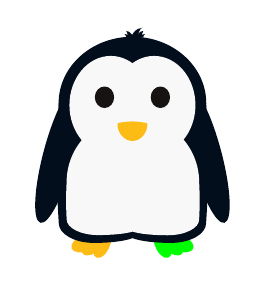
\begin{tikzpicture}
	\pingu[left foot color=green]
\end{tikzpicture}
\end{tcblisting}
\end{keyexplain}

\shortcuts{left foot}{\@pingu@leftfoot@}{left foot color}

\begin{keyexplain}{right foot}{foot-selector}{\@pingu@select@rightfoot@}
	Change the style of the right foot. All valid values are listed in \autoref{mrk:pengu-change-comps}.
\begin{tcblisting}{listing options={style=lstpingu,language=pingulang,deleteemph={[2]{simple}}}}

\begin{tikzpicture}
	\pingu[right foot=simple]
\end{tikzpicture}
\end{tcblisting}
\end{keyexplain}

\begin{keyexplain}{right foot color}{color}{\pingu@color@foot@right}
	Change the color of the right foot of the penguin.%
\begin{tcblisting}{}
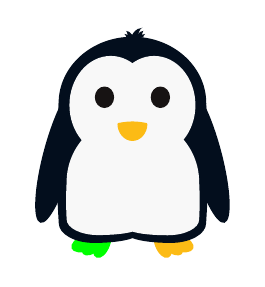
\begin{tikzpicture}
	\pingu[right foot color=green]
\end{tikzpicture}
\end{tcblisting}
\end{keyexplain}

\shortcuts{right foot}{\@pingu@rightfoot@}{right foot color}

\begin{keyexplain}{feet}{foot-selector}{}
	Change the style of both feet by calling \keyref{left foot} and \keyref{right foot} with the same value.
\begin{tcblisting}{listing options={style=lstpingu,language=pingulang,deleteemph={[2]{simple}}}}

\begin{tikzpicture}
	\pingu[feet=simple]
\end{tikzpicture}
\end{tcblisting}
\end{keyexplain}

\begin{keyexplain}{feet color}{color}{}
	Sets the color of both feet by calling \keyref{left foot color} and \keyref{right foot color} with the same value.
\begin{tcblisting}{}
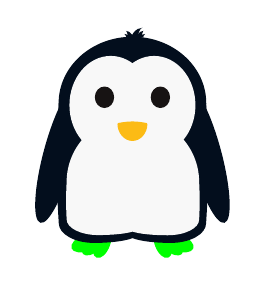
\begin{tikzpicture}
	\pingu[feet color=green]
\end{tikzpicture}
\end{tcblisting}
\end{keyexplain}

\shortcuts{feet}{\@pingu@leftfoot@}{feet color}

\subsubsection{The Body}
\begin{keyexplain}{body main}{color}{\pingu@color@body@main}
	Set the main color of the penguin. This will affect \keyref{hair} as well, as this chooses its default value from the main color.%
\begin{tcblisting}{}
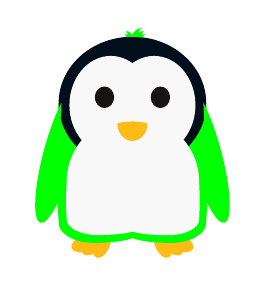
\begin{tikzpicture}
	\pingu[body main=green]
\end{tikzpicture}
\end{tcblisting}
\end{keyexplain}

\begin{keyexplain}{body head}{color}{\pingu@color@body@head}
	Set the color of the penguin head.%
\begin{tcblisting}{}
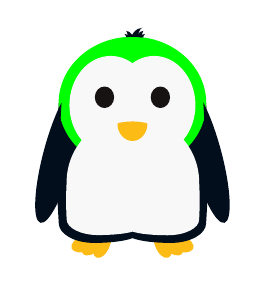
\begin{tikzpicture}
	\pingu[body head=green]
\end{tikzpicture}
\end{tcblisting}
\end{keyexplain}

\begin{keyexplain}{body}{color}{}
	Sets the color of the main penguin and the head, by calling \keyref{body main} and \keyref{body head} with the same value.
\begin{tcblisting}{}
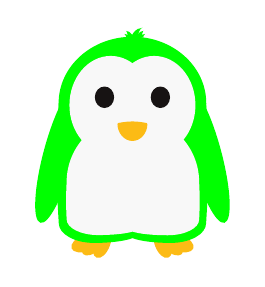
\begin{tikzpicture}
	\pingu[body=green]
\end{tikzpicture}
\end{tcblisting}
\end{keyexplain}

\begin{keyexplain}{body front}{color}{\pingu@color@body@front}
	Sets the frontal color of the penguin.
\begin{tcblisting}{}
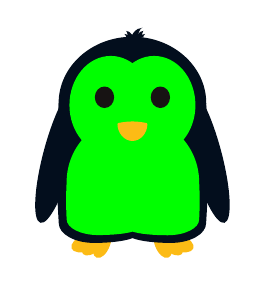
\begin{tikzpicture}
	\pingu[body front=green]
\end{tikzpicture}
\end{tcblisting}
\end{keyexplain}


\subsubsection{The Size}

\begin{keyexplain}{height}{length}{\the\pingu@side@h@half}
	Change the height of the penguin manually. You probably should not use this key directly and refer to \keyref{small size}, \keyref{normal size}, and \keyref{large size}:
\begin{tcblisting}{listing options={style=lstpingu,language=pingulang}}

\begin{tikzpicture}
	\pingu[height=17mm]
\end{tikzpicture}
\end{tcblisting}
\end{keyexplain}

\begin{keyexplain}{small size}{}{}
	Will use \keyref{height} to create a small pingu:
\begin{tcblisting}{listing options={style=lstpingu,language=pingulang}}

\begin{tikzpicture}
	\pingu[small size]
\end{tikzpicture}
\end{tcblisting}
\end{keyexplain}

\keyalias{small}{small size}
\keyalias{small height}{small size}

\begin{keyexplain}{normal size}{}{}
	Will use \keyref{height} to create a normal pingu:
\begin{tcblisting}{listing options={style=lstpingu,language=pingulang}}

\begin{tikzpicture}
	\pingu[normal size]
\end{tikzpicture}
\end{tcblisting}
\end{keyexplain}

\keyalias{normal}{normal size}
\keyalias{normal height}{normal size}

\begin{keyexplain}{large size}{}{}
	Will use \keyref{height} to create a large pingu:
\begin{tcblisting}{listing options={style=lstpingu,language=pingulang}}

\begin{tikzpicture}
	\pingu[large size]
\end{tikzpicture}
\end{tcblisting}
\end{keyexplain}

\keyalias{large}{large size}
\keyalias{large height}{large size}

\subsubsection{The Eyes}
\begin{keyexplain}{left eye}{eye-selector}{\@pingu@select@lefteye@}
	Change the style of the left eye. All valid values are listed in \autoref{mrk:pengu-eye}.
\begin{tcblisting}{listing options={style=lstpingu,language=pingulang,deleteemph={[2]{wink}}}}

\begin{tikzpicture}
	\pingu[left eye=wink]
\end{tikzpicture}
\end{tcblisting}
\end{keyexplain}

\begin{keyexplain}{left eye color}{color}{\pingu@color@eye@left}
	Change the main color of the left eye.
\begin{tcblisting}{}
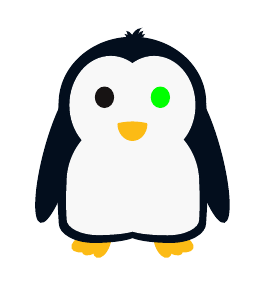
\begin{tikzpicture}
	\pingu[left eye color=green]
\end{tikzpicture}
\end{tcblisting}
\end{keyexplain}

\begin{keyexplain}{left eye second color}{color}{\pingu@color@eye@second@left}
	Change the secondary color of the left eye. It will be used in some styles selected by \keyref{left eye} (e.g. \textit{shiny}):
\begin{tcblisting}{listing options={style=lstpingu,language=pingulang,deleteemph={[2]{shiny}}}}
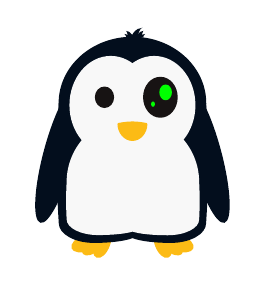
\begin{tikzpicture}
	\pingu[left eye=shiny,
	  left eye second color=green]
\end{tikzpicture}
\end{tcblisting}
\end{keyexplain}

\shortcuts{left eye}{\@pingu@lefteye@}{left eye color}

\begin{keyexplain}{right eye}{eye-selector}{\@pingu@select@righteye@}
	Change the style of the right eye. All valid values are listed in \autoref{mrk:pengu-eye}.
\begin{tcblisting}{listing options={style=lstpingu,language=pingulang,deleteemph={[2]{wink}}}}

\begin{tikzpicture}
	\pingu[right eye=wink]
\end{tikzpicture}
\end{tcblisting}
\end{keyexplain}

\begin{keyexplain}{right eye color}{color}{\pingu@color@eye@right}
	Change the main color of the right eye.
\begin{tcblisting}{}
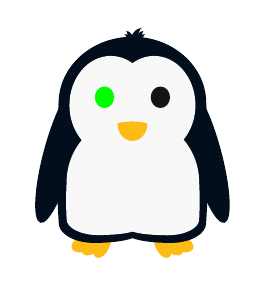
\begin{tikzpicture}
	\pingu[right eye color=green]
\end{tikzpicture}
\end{tcblisting}
\end{keyexplain}

\begin{keyexplain}{right eye second color}{color}{\pingu@color@eye@second@right}
	Change the secondary color of the right eye. It will be used in some styles selected by \keyref{right eye} (e.g. \textit{shiny}):
\begin{tcblisting}{listing options={style=lstpingu,language=pingulang,deleteemph={[2]{shock}}}}
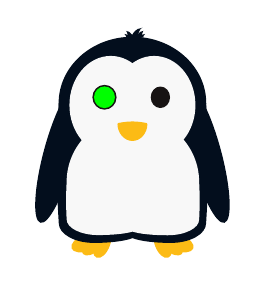
\begin{tikzpicture}
	\pingu[right eye=shock,
	  right eye second color=green]
\end{tikzpicture}
\end{tcblisting}
\end{keyexplain}

\shortcuts{right eye}{\@pingu@righteye@}{right eye color}

\begin{keyexplain}{eyes}{eye-selector}{}
	Change the style of both eyes by calling \keyref{left eye} and \keyref{right eye} with the same value.
\begin{tcblisting}{listing options={style=lstpingu,language=pingulang,deleteemph={[2]{wink}}}}

\begin{tikzpicture}
	\pingu[eyes=wink]
\end{tikzpicture}
\end{tcblisting}
\end{keyexplain}

\begin{keyexplain}{eyes color}{color}{}
	Change the main color of both eyes by calling \keyref{left eye color} and \keyref{right eye color} with the same value.
\begin{tcblisting}{}
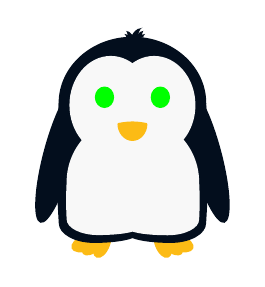
\begin{tikzpicture}
	\pingu[eyes color=green]
\end{tikzpicture}
\end{tcblisting}
\end{keyexplain}

\begin{keyexplain}{eyes second color}{color}{}
	Change the secondary color of  both eyes by calling \keyref{left eye second color} and \keyref{right eye second  color} with the same value.
\begin{tcblisting}{listing options={style=lstpingu,language=pingulang,deleteemph={[2]{shock,shiny}}}}
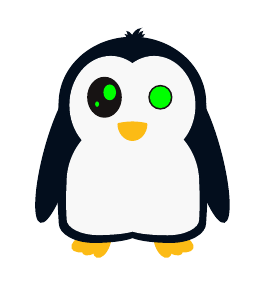
\begin{tikzpicture}
	\pingu[left eye=shock, right eye=shiny,
	  eyes second color=green]
\end{tikzpicture}
\end{tcblisting}
\end{keyexplain}

\shortcuts{eyes}{\@pingu@lefteye@}{eyes color}

\subsubsection{The Wings}

\begin{keyexplain}{left wing}{wing-selector}{\@pingu@select@leftwing@}
	Change the style of the left wing. All valid values are listed in \autoref{subsec:wings}.
\begin{tcblisting}{listing options={style=lstpingu,language=pingulang,deleteemph={[2]{wave}}}}

\begin{tikzpicture}
	\pingu[left wing=wave]
\end{tikzpicture}
\end{tcblisting}
\end{keyexplain}

\begin{keyexplain}{left wing color}{color}{\pingu@color@left@wing}
	Change the main color of the left wing.
\begin{tcblisting}{}
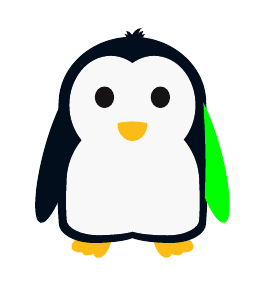
\begin{tikzpicture}
	\pingu[left wing color=green]
\end{tikzpicture}
\end{tcblisting}
\end{keyexplain}

\shortcuts{left wing}{\@pingu@leftwing@}{left wing color}

\begin{keyexplain}{right wing}{wing-selector}{\@pingu@select@rightwing@}
	Change the style of the right wing. All valid values are listed in \autoref{subsec:wings}.
\begin{tcblisting}{listing options={style=lstpingu,language=pingulang,deleteemph={[2]{wave}}}}
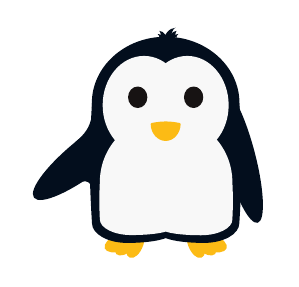
\begin{tikzpicture}
	\pingu[right wing=hug]
\end{tikzpicture}
\end{tcblisting}
\end{keyexplain}

\begin{keyexplain}{right wing color}{color}{\pingu@color@right@wing}
	Change the main color of the right wing.
\begin{tcblisting}{}
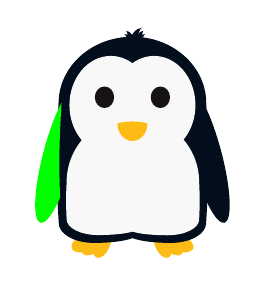
\begin{tikzpicture}
	\pingu[right wing color=green]
\end{tikzpicture}
\end{tcblisting}
\end{keyexplain}

\shortcuts{right wing}{\@pingu@rightwing@}{right wing color}

\begin{keyexplain}{wings}{wing-selector}{}
	Change the style of both wings by calling \keyref{left wing} and \keyref{right wing} with the same value.
\begin{tcblisting}{listing options={style=lstpingu,language=pingulang,deleteemph={[2]{wink}}}}

\begin{tikzpicture}
	\pingu[wings=grab]
\end{tikzpicture}
\end{tcblisting}
\end{keyexplain}

\begin{keyexplain}{wings color}{color}{}
	Change the main color of both wings by calling \keyref{left wing color} and \keyref{right wing color} with the same value.
\begin{tcblisting}{}
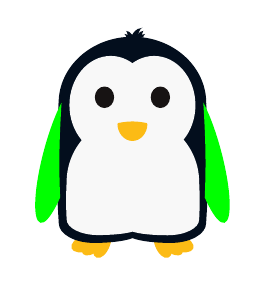
\begin{tikzpicture}
	\pingu[wings color=green]
\end{tikzpicture}
\end{tcblisting}
\end{keyexplain}

\shortcuts{wings}{\@pingu@leftwing@}{wings color}

\subsubsection{The Hair}
\begin{keyexplain}{hairstyle}{hair-selector}{\@pingu@select@hairstyle@}
	Change the hairstyle (\autoref{mrk:pengu-change-comps}):
\begin{tcblisting}{}

\begin{tikzpicture}
	\pingu[hairstyle=none]
\end{tikzpicture}
\end{tcblisting}
\end{keyexplain}

\keyalias{hair style}{hairstyle}
% \shortcuts{hair}{\@pingu@hairstyle@}{wings color}

\begin{keyexplain}{hair 1 color}{color}{\pingu@color@hair@a}
	Set the color of the first hair (this may be used differently by other hairstyles):
\begin{tcblisting}{listing options={style=lstpingu,language=pingulang,moreemph={[2]{1}}}}
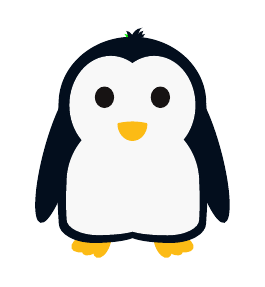
\begin{tikzpicture}
	\pingu[hair 1 color=green]
\end{tikzpicture}
\end{tcblisting}
\end{keyexplain}

\begin{keyexplain}{hair 2 color}{color}{\pingu@color@hair@b}
	Set the color of the second hair (this may be used differently by other hairstyles):
\begin{tcblisting}{listing options={style=lstpingu,language=pingulang,moreemph={[2]{2}}}}
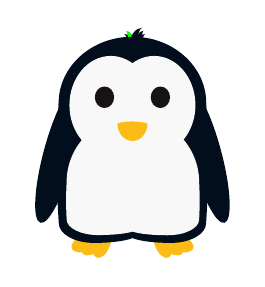
\begin{tikzpicture}
	\pingu[hair 2 color=green]
\end{tikzpicture}
\end{tcblisting}
\end{keyexplain}

\begin{keyexplain}{hair 3 color}{color}{\pingu@color@hair@c}
	Set the color of the third hair (this may be used differently by other hairstyles):
\begin{tcblisting}{listing options={style=lstpingu,language=pingulang,moreemph={[2]{3}}}}
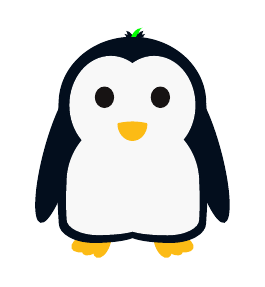
\begin{tikzpicture}
	\pingu[hair 3 color=green]
\end{tikzpicture}
\end{tcblisting}
\end{keyexplain}

\begin{keyexplain}{hair 4 color}{color}{\pingu@color@hair@d}
	Set the color of the fourth hair (this may be used differently by other hairstyles):
\begin{tcblisting}{listing options={style=lstpingu,language=pingulang,moreemph={[2]{4}}}}
\begin{tikzpicture}
	\pingu[hair 4 color=green]
\end{tikzpicture}
\end{tcblisting}
\end{keyexplain}

\begin{keyexplain}{hair 5 color}{color}{\pingu@color@hair@e}
	Set the color of the fifth hair (this may be used differently by other hairstyles):
\begin{tcblisting}{listing options={style=lstpingu,language=pingulang,moreemph={[2]{5}}}}
\begin{tikzpicture}
	\pingu[hair 5 color=green]
\end{tikzpicture}
\end{tcblisting}
\end{keyexplain}

\begin{keyexplain}{hairs color}{color}{}
	Set the color of all hairs by calling \keyref{hair 1 color}, \keyref{hair 2 color}, \keyref{hair 3 color}, \keyref{hair 4 color}, and \keyref{hair 5 color} with the same argument:
\begin{tcblisting}{}
\begin{tikzpicture}
	\pingu[hairs color=green]
\end{tikzpicture}
\end{tcblisting}
\end{keyexplain}

\keyalias{hairs}{hairs color}
\keyalias{hair}{hairs color}

\subsubsection{The Bill}
\begin{keyexplain}{bill}{bill-selector}{\@pingu@select@bill@}
	Change the style of the bill (\autoref{mrk:pengu-change-comps}):
\begin{tcblisting}{listing options={style=lstpingu,language=pingulang,deleteemph={[2]{flat}}}}
\begin{tikzpicture}
	\pingu[bill=flat]
\end{tikzpicture}
\end{tcblisting}
\end{keyexplain}

\begin{keyexplain}{bill color}{color}{\pingu@color@bill}
	Change the color of the bill
\begin{tcblisting}{}
\begin{tikzpicture}
	\pingu[bill color=green]
\end{tikzpicture}
\end{tcblisting}
\end{keyexplain}

\subsection{Drawing Styles}
\index{Styles}
\def\cursub{Styles!}
\begin{keyexplain}{:line}{}{}
	Disable glows, shades and fills and enforce a line. This line will be darker
	than the original fill color:
\begin{tcblisting}{}
\begin{tikzpicture}
	\pingu[:line]
\end{tikzpicture}
\end{tcblisting}
\end{keyexplain}

\begin{keyexplain}{:ghost parts}{opacity}{.5}
	Set the opacity of each penguin component individually. At the moment, this
	excludes some glow calculations.
\begin{tcblisting}{}
\begin{tikzpicture}
	\pingu[:ghost parts]
\end{tikzpicture}
\end{tcblisting}
\end{keyexplain}

\begin{keyexplain}{:ghost}{opacity}{.5}
	Set the opacity of the complete penguin. At the moment, this
	excludes some glow calculations.
\begin{tcblisting}{}
\begin{tikzpicture}
	\pingu[:ghost]
\end{tikzpicture}
\end{tcblisting}
\end{keyexplain}

\begin{keyexplain}{:devil}{color}{pingu@purple}
	Enable all devil components and set their main color:
\begin{tcblisting}{}
\begin{tikzpicture}
	\pingu[:devil=green]
\end{tikzpicture}
\end{tcblisting}
\end{keyexplain}

\begin{keyexplain}{:back}{}{}
	Mirror the penguin, this swaps left and right, the rotation and more.
	Yet, at least at the time of writing, this does not swap the drawing order in each layer, but just the layers:\typeout{KTWKKS}
\begin{tcblisting}{}
\begin{tikzpicture}
	\pingu[:back, left wing wave,
	       cane left, left item angle=70]
\end{tikzpicture}
\end{tcblisting}
\end{keyexplain}

\def\cursub{}

\subsection{Extras}

\begin{keyexplain}{tie}{color}{pingu@green}
	Enable the tie extra:
\begin{tcblisting}{}
\begin{tikzpicture}
	\pingu[tie]
\end{tikzpicture}
\end{tcblisting}
\end{keyexplain}

{\def\pingu@color@tie{<tie-color>}
\begin{subkeyexplain}{tie}{tie knot}{color}{\pingu@color@tie@knot}
	Change the tie knot:
\begin{tcblisting}{}
\begin{tikzpicture}
	\pingu[tie, tie knot=orange]
\end{tikzpicture}
\end{tcblisting}
\end{subkeyexplain}
}


\subsection{Wing-Items}
\label{sub:wing-items}

\begin{keyexplain}{left wing item angle}{angle}{\pingu@wing@left@item@angle@user}
	Relative rotation of the \hyperref[sub:wing-items]{wing items} placed in the left wing:
\begin{tcblisting}{}
\begin{tikzpicture}
	\pingu[cane left, cane right,
	       left wing item angle=70]
\end{tikzpicture}
\end{tcblisting}
\end{keyexplain}

\keyalias{left item angle}{left wing item angle}

\begin{keyexplain}{left wing item flip}{true/false}{\if@pingu@wi@flip@left true\else false\fi}
	Some \hyperref[sub:wing-items]{wing items} do have a different style, depending on the wing they are in (e.g. they are mirrored). This option toggles the stile for the left wing.
\begin{tcblisting}{}
\begin{tikzpicture}
	\pingu[flag left, flag right,
				 left wing item flip]
\end{tikzpicture}
\end{tcblisting}
\end{keyexplain}

\keyalias{left item flip}{left wing item flip}

\begin{keyexplain}{right wing item angle}{angle}{\pingu@wing@right@item@angle@user}
	Relative rotation of the \hyperref[sub:wing-items]{wing items} placed in the right wing:
\begin{tcblisting}{}
\begin{tikzpicture}
	\pingu[cane left, cane right,
	       right wing item angle=70]
\end{tikzpicture}
\end{tcblisting}
\end{keyexplain}

\keyalias{right item angle}{right wing item angle}

\begin{keyexplain}{right wing item flip}{true/false}{\if@pingu@wi@flip@right true\else false\fi}
	Some \hyperref[sub:wing-items]{wing items} do have a different style, depending on the wing they are in (e.g. they are mirrored). This option toggles the stile for the right wing.
\begin{tcblisting}{}
\begin{tikzpicture}
	\pingu[flag left, flag right,
				 right wing item flip]
\end{tikzpicture}
\end{tcblisting}
\end{keyexplain}

\keyalias{right item flip}{right wing item flip}

\subsection{Clothes}

\printindex

\end{document}